
% Created by Bonita Graham
% Last update: December 2019 By Kestutis Bendinskas

% Authors: 
% Please do not make changes to the preamble until after the solid line of %s.

\documentclass[10pt]{article}
\usepackage[explicit]{titlesec}
\setlength{\parindent}{0pt}
\setlength{\parskip}{1em}
\usepackage{hyphenat}
\usepackage{ragged2e}
\RaggedRight

% These commands change the font. If you do not have Garamond on your computer, you will need to install it.
\usepackage{garamondx}
\usepackage[T1]{fontenc}
\usepackage{amsmath, amsthm}
\usepackage{graphicx}

\usepackage{mathtools}
\DeclarePairedDelimiter\ceil{\lceil}{\rceil}
\DeclarePairedDelimiter\floor{\lfloor}{\rfloor}

\usepackage{xcolor} % Define custom colours using \textcolor{color}{text}
\usepackage{float}

% Colour definitions
\definecolor{darkpink}{rgb}{1.0, 0.13, 0.32}

% This adjusts the underline to be in keeping with word processors.
\usepackage{soul}
\setul{.6pt}{.4pt}


% The following sets margins to 1 in. on top and bottom and .75 in on left and right, and remove page numbers.
\usepackage{geometry}
\geometry{vmargin={1in,1in}, hmargin={.75in, .75in}}
\usepackage{fancyhdr}
\pagestyle{fancy}
\pagenumbering{gobble}
\renewcommand{\headrulewidth}{0.0pt}
\renewcommand{\footrulewidth}{0.0pt}

% These Commands create the label style for tables, figures and equations.
\usepackage[labelfont={footnotesize,bf} , textfont=footnotesize]{caption}
\captionsetup{labelformat=simple, labelsep=period}
\newcommand\num{\addtocounter{equation}{1}\tag{\theequation}}
\renewcommand{\theequation}{\arabic{equation}}
\makeatletter
\renewcommand\tagform@[1]{\maketag@@@ {\ignorespaces {\footnotesize{\textbf{Equation}}} #1.\unskip \@@italiccorr }}
\makeatother
\setlength{\intextsep}{10pt}
\setlength{\abovecaptionskip}{2pt}
\setlength{\belowcaptionskip}{-10pt}

\renewcommand{\textfraction}{0.10}
\renewcommand{\topfraction}{0.85}
\renewcommand{\bottomfraction}{0.85}
\renewcommand{\floatpagefraction}{0.90}

% These commands set the paragraph and line spacing
\titleformat{\section}
  {\normalfont}{\thesection}{1em}{\MakeUppercase{\textbf{#1}}}
\titlespacing\section{0pt}{0pt}{-10pt}
\titleformat{\subsection}
  {\normalfont}{\thesubsection}{1em}{\textit{#1}}
\titlespacing\subsection{0pt}{0pt}{-8pt}
\renewcommand{\baselinestretch}{1.15}

% This designs the title display style for the maketitle command
\makeatletter
\newcommand\sixteen{\@setfontsize\sixteen{17pt}{6}}
\renewcommand{\maketitle}{\bgroup\setlength{\parindent}{0pt}
\begin{flushleft}
\sixteen\bfseries \@title
\medskip
\end{flushleft}
\textit{\@author}
\egroup}
\makeatother

% This styles the bibliography and citations.
%\usepackage[biblabel]{cite}
\usepackage[sort&compress]{natbib}
\setlength\bibindent{2em}
\makeatletter
\renewcommand\@biblabel[1]{\textbf{#1.}\hfill}
\makeatother
\renewcommand{\citenumfont}[1]{\textbf{#1}}
\bibpunct{}{}{,~}{s}{,}{,}
\setlength{\bibsep}{0pt plus 0.3ex}




%%%%%%%%%%%%%%%%%%%%%%%%%%%%%%%%%%%%%%%%%%%%%%%%%

% Authors: Add additional packages and new commands here.  
% Limit your use of new commands and special formatting.

% Place your title below. Use Title Capitalization.
\title{Final assignment ROS01}

% Add author information below. Communicating author is indicated by an asterisk, the affiliation is shown by superscripted lower case letter if several affiliations need to be noted.
\author{
Youri Klaassens$^{a}$, Nick van Endhoven$^{b}$ \\ \medskip 
$^{a}$student Computer Engineering Rotterdam University of Applied Science, 0996211@hr.nl, Zwaag \\ 
$^{b}$student Computer Engineering Rotterdam University of Applied Science, 0998831@hr.nl, Breda\\ \medskip 
}

\pagestyle{empty}
\begin{document}

% Makes the title and author information appear.
\vspace*{.01 in}
\maketitle
\vspace{.12 in}

% Introduction.
\section*{introduction}

\begin{table}[H]
    \centering
    \begin{tabular}{|l|c|c|c|}
        \hline
        \textcolor{darkpink}{\textit{Task}}& \textcolor{darkpink}{\textit{Arrival time}} & \textcolor{darkpink}{\textit{BC deadline}} &  \textcolor{darkpink}{\textit{WC deadline}} \\
        \hline
        \textbf{Compass} & 200 ms $ \pm $ 20 ms & 5 ms & 35 ms \\
        \hline
        \textbf{Airbag} & 3000 ms $ \pm $ 1500 ms & 30 ms & 32 ms \\
        \hline
        \textbf{GPS} & 1300 ms $ \pm $ 20 ms & 5 ms & 70 ms \\
        \hline
    \end{tabular}

    \caption{Characteristics of the available shared resources. }
    \label{tab:resource_characteristics}
\end{table}

\section*{Implementation}
\newpage

\section*{Results}

\begin{figure}[H]
\caption{Result without shared UART resource}
\label{resNoUART}
\centering
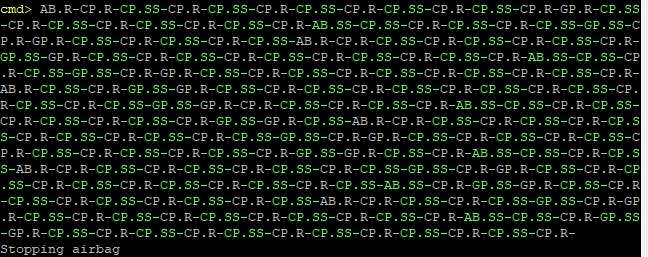
\includegraphics[width=0.7\linewidth]{./images/result_no_uart.jpeg}
\end{figure}

\begin{figure}[H]
\caption{Result with shared UART resource}
\label{res}
\centering
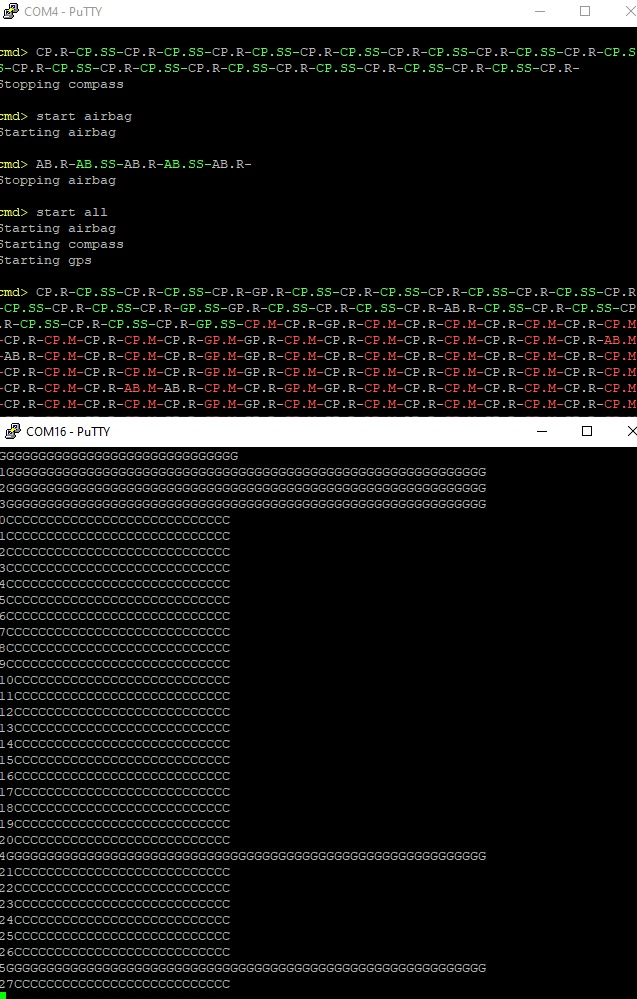
\includegraphics[width=0.7\linewidth]{./images/result.jpeg}
\end{figure}
\newpage

\section*{Conclusion}
\newpage
\end{document}
